\section{Ломаные и $\epsilon$-приближения}

\mysubsection{Изображение графов}

	Ранее во втором разделе мы уже говорили, что когда мы рисуем граф на плоскости и говорим, например, что это полный граф на $n$ вершинах, то мы немного лукавим: в действительности это только изображение графа. Сам же граф навсегда останется только абстрактным понятием.
	
	Оказываетя, что теория, исследующая способы <<рисовать>> графы, не лишена смысла. Ведь по отличиям в рисунке можно судить и о различиях в самих графах. Однако тут все не так просто, как и во всей математике, потому что возникает необходимость очень дотошно подходить к этому вопросу, иначе при переходе к более абстрактным объектам мы не сможем понять, почему те или иные изображения невозможны при определенных условиях. 
	
	Везде далее мы будем подразумевать, что графы у нас только неориентированные.

\begin{center}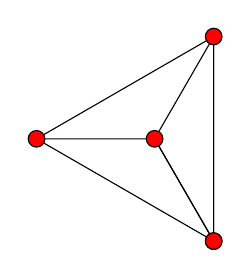
\begin{tikzpicture}
	\tikzstyle{every node}=[circle, draw, fill=red, inner sep=0pt, minimum width=6pt]
	\foreach \x in {-60,60,...,300}
    {
    	\draw (\x + 120:1.5) -- (\x:1.5) -- (0, 0);
    };
    \foreach \x in {-60,60,...,300}
    {
    	\draw (\x:1.5) node {};
    };
    \draw (0, 0) node {};
\end{tikzpicture}\; \; \; \; \; \; \; \; \; \; 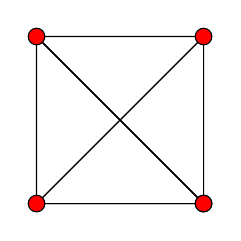
\begin{tikzpicture}
	\tikzstyle{every node}=[circle, draw, fill=red, inner sep=0pt, minimum width=6pt]
	\foreach \x in {-45,45,...,315}
    {
    	\draw (\x + 180:1.5) -- (\x:1.5) -- (\x-90:1.5);
    };
    \foreach \x in {-45,45,...,315}
    {
    	\draw (\x:1.5) node {};
    };
\end{tikzpicture}

	\small Рис. \images. Две реализации графа $K_4$ на плоскости
\end{center}

	Даже говоря о графах на рисунке выше мы можем сказать, что они изоморфны, но при этом их некоторые <<утолщения>> не будут изоморфными. Дадим точное определение изображения графа на плоскости.
	
\begin{definition}
	Ограниченное непустое множество $E \subset \BR^2$ называется \emph{изображением графа $G$} на плоскости, если существует набор точек $\lbrace x_k \rbrace_{k=1}^{|V|}$, которому поставлен в соответствие набор вершин ($x_k \leftrightarrow v_k \in V(G)$) так, что ребро $e = \lbrace v_s, v_t \rbrace$ лежит в $E(G)$ тогда и только тогда, когда существует кусочно непрерывная функция $f_e(t), t \in [0, 1]$, обладающая следующими свойствами:
\begin{itemize}
	\item $f_e(0) = x_s, f_e(1) = x_t$,
	\item $\forall \!\ t \in (0, 1) \mapsto f_e(t) \in E$,
	\item $\forall \!\ f_{e_1}, f_{e_2}, e_1 \neq e_2 \mapsto \nexists t_1  \in (0, 1), t_2 \in (0, 1) \colon f_{e_1}(t_1) = f_{e_2}(t_2)$.
\end{itemize}
	И при этом любая точка $x \in E$ является точкой какой-то функции $f_e(t)$ или точкой из набора $\lbrace x_k \rbrace_{k=1}^{|V|}$.
\end{definition}

	Не стоит пугаться такого ужасного длинного определения. Оно содержит так много строк в себе, потому что мы на языке математике пробуем задать то, что интуитивно понимаем, когда видим граф, нарисованным в учебнике, на доске или где-нибудь еще.

	Теперь мы можем переопределить планарность графа.
	
\begin{definition}
	Граф \emph{планарен}, если существует его изображение, в котором все функции $f_e(t)$ непрерывныи кусочно линейны.
\end{definition}

	То есть планарным графом теперь юудет тот, у которого есть изображение, на котором все ребра изображены в виде ломаных, которые нигде не пересекаются, кроме, быть может, концов. Так же мы будем говорить о плоском графе, что он реализуем на плоскости.

\mysubsection{Общее положение}

	И вот тут мы натыкаемся на еще одну высокую преграду в реализации каких-то объектов на плоскости, а именно, нам придется доказывать некоторые интуитивно понятные вещи очень сложно, потому что таково их строгое доказательство.

\begin{definition}
	Будем говорить, что множество точек $\lbrace x_k \rbrace_{k = 1}^{n}$ находится \emph{в общем положении}, если любые три точки не лежат на одной прямой и любые три отрезка, их соединяющие, не пересекаются в одной точке.
\end{definition}

	Свойство набора точек быть в общем положении важно, потому что сейчас мы будем решать комбинаторные задачи, в которых будет важно число пересечений отрезков между собой. Если точки находятся в общем положении, то число таких пересечений либо сложно вычислить, либо невозможно.
	
\begin{statement}
	На плоскости даны два треугольника $\vartriangle ABC$ и $\vartriangle A'B'C'$. Известно, что все шесть вершин этих треугольников находятся в общем положении, докажите, что контуры этих треугольников будут пересекаться в четном числе точек.
	
\begin{proof}
	Сначала зафиксируем $\vartriangle A'B'C'$ и будем рассматривать возможное расположение других трех точек. Сделаем сразу замечание, что в силу общего положения мы рассматриваем только случаи, когда для любой прямой, проходящей черзе две точки, все остальные точки строго попадают в одну или другую открытые полуплоскости.
	
\begin{paracol}{2}
	Допустим, что внутрь попала хотя бы одна точка. Обозначим ее $A$. Если все остальные точки тоже попали внутрь, то пересечений нет, то есть их число "--- $0$ (четное). Иначе есть вершина вне треугольника, обозначим ее $B$ и предположим, что она пересекает сторону $B'C'$ (от этого общность решения не уменьшится). Теперь проведем все четыре прямых, содержащие стороны треугольника и отрезок $AB$, они разобьют плоскость на несколько фрагментов. Простым перебором можно убедиться, что в какую бы часть плоскости не попала бы вершина $C$, то число пересечений всегда будет четно.
	
\switchcolumn

\begin{center}
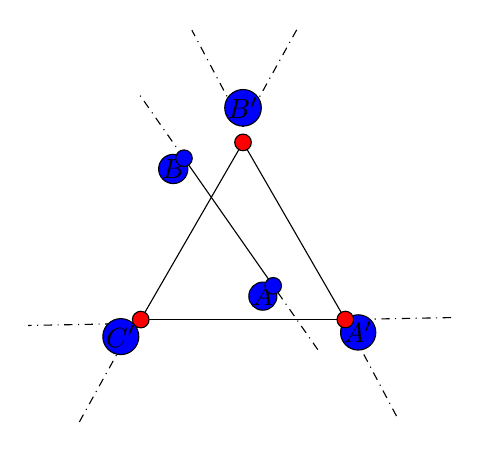
\begin{tikzpicture}
	
	\coordinate (A') at (-30:1.5);
	\coordinate (B') at (90:1.7);	
	\coordinate (C') at (210:1.6);	
	\coordinate (A) at (-40:0.5);
	\coordinate (B) at (120:1.5);	
	
	\foreach \x in {-30,90,210}
    {
    	\draw (\x + 120:1.5) -- (\x:1.5);
    };
    \foreach \a/\b in {A/B,A'/B',C'/B',A'/C'}
    {
		\path (\a) -- (\b) coordinate[pos=-0.5](l) coordinate[pos=1.5](r);
		\draw [dash dot](l) -- (\a) [dash dot](\b) -- (r);
	};
	
    \draw (A') node [below right]{$A'$};
    \draw (B') node [above]{$B'$};
    \draw (C') node [below left]{$C'$};
    \draw (A) node [below left]{$A$};
    \draw (B) node [below left]{$B$};
    
    \tikzstyle{every node}=[circle, draw, fill=red, inner sep=0pt, minimum width=6pt]
    \foreach \x in {-30,90,210}
    {
    	\draw (\x:1.5) node {};
    };
    \tikzstyle{every node}=[circle, draw, fill=blue, inner sep=0pt, minimum width=6pt]
    \draw (-40:0.5) node {} -- (120:1.5) node {};
    
\end{tikzpicture}\end{center}
\begin{center}
	\small Рис. \images. 
\end{center}
\end{paracol}	
	
	Теперь предположим, что все вершины находятся вне этого треугольника. Тогда если какой-нибудь отрезок контура $\vartriangle ABC$ и пересекает $\vartriangle A'B'C'$, то обязательно в двух точках, иначе мы получили бы предыдущий случай. Суммируя, имеем, что контуры пересекаются в четном числе точек 
\end{proof} 
\end{statement}

\begin{consequence}
	Если на плоскости есть $2k + 2$ точки в общем положении ($k = m + n, m \in \BN, n \in \BN$), причем ровно $2m + 1$ вершина красного цвета и $2n + 1$ вершина синего цвета, тогда число пересечений отрезков, соединяющих две красные точки, с отрезками, соединяющими две синие точки, четно.
	
\begin{proof}
	Рассмотрим все красные и все синие треугольники и просуммируем число их пересечеений, получим $S$. В силу того, что число попарных пересечений четно, $S$ тоже четно.
	
	Давайте рассмотрим теперь пару пересекающихся отрезков разного цвета. Это пересечение учитывалось ровно в $(2n-1) \cdot (2m-1)$ треугольниках, то есть в нечетном их числе. Тогда если бы было нечетное число пересечений, то $S$ было бы нечетно. Противоречие.
\end{proof}
\end{consequence}

\mysubsection{Ломаные. Утолщения}

	Сейчас мы подойдем наиболее близко к математическому анализу. Наша цель явно показать, что, рисуя на плоскости какую-то ломаную, мы не можем получить сложную фигуру. Более того, для любой ломаной мы можем построить достаточно близкую к ней ломаную, которая будет обладать к тому же некоторыми приятными свойствами. Подробнее обо всем этом написано ниже. 